
%% bisturbile_defence_matrix.tex
%% V1.4b
%% 2015/08/26
%% by Michael Shell
%% See:
%% http://www.michaelshell.org/
%% for current contact information.
%%
%% This is a skeleton file demonstrating the advanced use of IEEEtran.cls
%% (requires IEEEtran.cls version 1.8b or later) with an IEEE Computer
%% Society journal paper.
%%
%% Support sites:
%% http://www.michaelshell.org/tex/ieeetran/
%% http://www.ctan.org/pkg/ieeetran
%% and
%% http://www.ieee.org/

%%*************************************************************************
%% Legal Notice:
%% This code is offered as-is without any warranty either expressed or
%% implied; without even the implied warranty of MERCHANTABILITY or
%% FITNESS FOR A PARTICULAR PURPOSE!
%% User assumes all risk.
%% In no event shall the IEEE or any contributor to this code be liable for
%% any damages or losses, including, but not limited to, incidental,
%% consequential, or any other damages, resulting from the use or misuse
%% of any information contained here.
%%
%% All comments are the opinions of their respective authors and are not
%% necessarily endorsed by the IEEE.
%%
%% This work is distributed under the LaTeX Project Public License (LPPL)
%% ( http://www.latex-project.org/ ) version 1.3, and may be freely used,
%% distributed and modified. A copy of the LPPL, version 1.3, is included
%% in the base LaTeX documentation of all distributions of LaTeX released
%% 2003/12/01 or later.
%% Retain all contribution notices and credits.
%% ** Modified files should be clearly indicated as such, including  **
%% ** renaming them and changing author support contact information. **
%%*************************************************************************


% *** Authors should verify (and, if needed, correct) their LaTeX system  ***
% *** with the testflow diagnostic prior to trusting their LaTeX platform ***
% *** with production work. The IEEE's font choices and paper sizes can   ***
% *** trigger bugs that do not appear when using other class files.       ***                          ***
% The testflow support page is at:
% http://www.michaelshell.org/tex/testflow/


% IEEEtran V1.7 and later provides for these CLASSINPUT macros to allow the
% user to reprogram some IEEEtran.cls defaults if needed. These settings
% override the internal defaults of IEEEtran.cls regardless of which class
% options are used. Do not use these unless you have good reason to do so as
% they can result in nonIEEE compliant documents. User beware. ;)
%
%\newcommand{\CLASSINPUTbaselinestretch}{1.0} % baselinestretch
%\newcommand{\CLASSINPUTinnersidemargin}{1in} % inner side margin
%\newcommand{\CLASSINPUToutersidemargin}{1in} % outer side margin
%\newcommand{\CLASSINPUTtoptextmargin}{1in}   % top text margin
%\newcommand{\CLASSINPUTbottomtextmargin}{1in}% bottom text margin




%
\documentclass[10pt,journal,compsoc]{IEEEtran}
% If IEEEtran.cls has not been installed into the LaTeX system files,
% manually specify the path to it like:
% \documentclass[10pt,journal,compsoc]{../sty/IEEEtran}


% For Computer Society journals, IEEEtran defaults to the use of
% Palatino/Palladio as is done in IEEE Computer Society journals.
% To go back to Times Roman, you can use this code:
%\renewcommand{\rmdefault}{ptm}\selectfont


% Some very useful LaTeX packages include:
% (uncomment the ones you want to load)



% *** MISC UTILITY PACKAGES ***
%
%\usepackage{ifpdf}
% Heiko Oberdiek's ifpdf.sty is very useful if you need conditional
% compilation based on whether the output is pdf or dvi.
% usage:
% \ifpdf
%   % pdf code
% \else
%   % dvi code
% \fi
% The latest version of ifpdf.sty can be obtained from:
% http://www.ctan.org/pkg/ifpdf
% Also, note that IEEEtran.cls V1.7 and later provides a builtin
% \ifCLASSINFOpdf conditional that works the same way.
% When switching from latex to pdflatex and vice-versa, the compiler may
% have to be run twice to clear warning/error messages.



% *** CITATION PACKAGES ***
%
\ifCLASSOPTIONcompsoc
  % The IEEE Computer Society needs nocompress option
  % requires cite.sty v4.0 or later (November 2003)
  \usepackage[nocompress]{cite}
\else
  % normal IEEE
  \usepackage{cite}
\fi
% cite.sty was written by Donald Arseneau
% V1.6 and later of IEEEtran pre-defines the format of the cite.sty package
% \cite{} output to follow that of the IEEE. Loading the cite package will
% result in citation numbers being automatically sorted and properly
% "compressed/ranged". e.g., [1], [9], [2], [7], [5], [6] without using
% cite.sty will become [1], [2], [5]--[7], [9] using cite.sty. cite.sty's
% \cite will automatically add leading space, if needed. Use cite.sty's
% noadjust option (cite.sty V3.8 and later) if you want to turn this off
% such as if a citation ever needs to be enclosed in parenthesis.
% cite.sty is already installed on most LaTeX systems. Be sure and use
% version 5.0 (2009-03-20) and later if using hyperref.sty.
% The latest version can be obtained at:
% http://www.ctan.org/pkg/cite
% The documentation is contained in the cite.sty file itself.
%
% Note that some packages require special options to format as the Computer
% Society requires. In particular, Computer Society  papers do not use
% compressed citation ranges as is done in typical IEEE papers
% (e.g., [1]-[4]). Instead, they list every citation separately in order
% (e.g., [1], [2], [3], [4]). To get the latter we need to load the cite
% package with the nocompress option which is supported by cite.sty v4.0
% and later.





% *** GRAPHICS RELATED PACKAGES ***
%

%\ifCLASSINFOpdf
\usepackage{graphicx}
%\DeclareGraphicsExtensions{.pdf,.jpeg,.png}
%\else
%  % or other class option (dvipsone, dvipdf, if not using dvips). graphicx
%  % will default to the driver specified in the system graphics.cfg if no
%  % driver is specified.
%  % \usepackage[dvips]{graphicx}
%  % declare the path(s) where your graphic files are
%  % \graphicspath{{../eps/}}
%  % and their extensions so you won't have to specify these with
%  % every instance of \includegraphics
%  % \DeclareGraphicsExtensions{.eps}
%\fi
% graphicx was written by David Carlisle and Sebastian Rahtz. It is
% required if you want graphics, photos, etc. graphicx.sty is already
% installed on most LaTeX systems. The latest version and documentation
% can be obtained at:
% http://www.ctan.org/pkg/graphicx
% Another good source of documentation is "Using Imported Graphics in
% LaTeX2e" by Keith Reckdahl which can be found at:
% http://www.ctan.org/pkg/epslatex
%
% latex, and pdflatex in dvi mode, support graphics in encapsulated
% postscript (.eps) format. pdflatex in pdf mode supports graphics
% in .pdf, .jpeg, .png and .mps (metapost) formats. Users should ensure
% that all non-photo figures use a vector format (.eps, .pdf, .mps) and
% not a bitmapped formats (.jpeg, .png). The IEEE frowns on bitmapped formats
% which can result in "jaggedy"/blurry rendering of lines and letters as
% well as large increases in file sizes.
%
% You can find documentation about the pdfTeX application at:
% http://www.tug.org/applications/pdftex





% *** MATH PACKAGES ***
%
%\usepackage{amsmath}
% A popular package from the American Mathematical Society that provides
% many useful and powerful commands for dealing with mathematics.
%
% Note that the amsmath package sets \interdisplaylinepenalty to 10000
% thus preventing page breaks from occurring within multiline equations. Use:
%\interdisplaylinepenalty=2500
% after loading amsmath to restore such page breaks as IEEEtran.cls normally
% does. amsmath.sty is already installed on most LaTeX systems. The latest
% version and documentation can be obtained at:
% http://www.ctan.org/pkg/amsmath





% *** SPECIALIZED LIST PACKAGES ***
%\usepackage{acronym}
% acronym.sty was written by Tobias Oetiker. This package provides tools for
% managing documents with large numbers of acronyms. (You don't *have* to
% use this package - unless you have a lot of acronyms, you may feel that
% such package management of them is bit of an overkill.)
% Do note that the acronym environment (which lists acronyms) will have a
% problem when used under IEEEtran.cls because acronym.sty relies on the
% description list environment - which IEEEtran.cls has customized for
% producing IEEE style lists. A workaround is to declared the longest
% label width via the IEEEtran.cls \IEEEiedlistdecl global control:
%
% \renewcommand{\IEEEiedlistdecl}{\IEEEsetlabelwidth{SONET}}
% \begin{acronym}
%
% \end{acronym}
% \renewcommand{\IEEEiedlistdecl}{\relax}% remember to reset \IEEEiedlistdecl
%
% instead of using the acronym environment's optional argument.
% The latest version and documentation can be obtained at:
% http://www.ctan.org/pkg/acronym


%\usepackage{algorithmic}
% algorithmic.sty was written by Peter Williams and Rogerio Brito.
% This package provides an algorithmic environment fo describing algorithms.
% You can use the algorithmic environment in-text or within a figure
% environment to provide for a floating algorithm. Do NOT use the algorithm
% floating environment provided by algorithm.sty (by the same authors) or
% algorithm2e.sty (by Christophe Fiorio) as the IEEE does not use dedicated
% algorithm float types and packages that provide these will not provide
% correct IEEE style captions. The latest version and documentation of
% algorithmic.sty can be obtained at:
% http://www.ctan.org/pkg/algorithms
% Also of interest may be the (relatively newer and more customizable)
% algorithmicx.sty package by Szasz Janos:
% http://www.ctan.org/pkg/algorithmicx




% *** ALIGNMENT PACKAGES ***
%
%\usepackage{array}
% Frank Mittelbach's and David Carlisle's array.sty patches and improves
% the standard LaTeX2e array and tabular environments to provide better
% appearance and additional user controls. As the default LaTeX2e table
% generation code is lacking to the point of almost being broken with
% respect to the quality of the end results, all users are strongly
% advised to use an enhanced (at the very least that provided by array.sty)
% set of table tools. array.sty is already installed on most systems. The
% latest version and documentation can be obtained at:
% http://www.ctan.org/pkg/array


%\usepackage{mdwmath}
%\usepackage{mdwtab}
% Also highly recommended is Mark Wooding's extremely powerful MDW tools,
% especially mdwmath.sty and mdwtab.sty which are used to format equations
% and tables, respectively. The MDWtools set is already installed on most
% LaTeX systems. The lastest version and documentation is available at:
% http://www.ctan.org/pkg/mdwtools


% IEEEtran contains the IEEEeqnarray family of commands that can be used to
% generate multiline equations as well as matrices, tables, etc., of high
% quality.


%\usepackage{eqparbox}
% Also of notable interest is Scott Pakin's eqparbox package for creating
% (automatically sized) equal width boxes - aka "natural width parboxes".
% Available at:
% http://www.ctan.org/pkg/eqparbox




% *** SUBFIGURE PACKAGES ***
%\ifCLASSOPTIONcompsoc
%  \usepackage[caption=false,font=footnotesize,labelfont=sf,textfont=sf]{subfig}
%\else
%  \usepackage[caption=false,font=footnotesize]{subfig}
%\fi
% subfig.sty, written by Steven Douglas Cochran, is the modern replacement
% for subfigure.sty, the latter of which is no longer maintained and is
% incompatible with some LaTeX packages including fixltx2e. However,
% subfig.sty requires and automatically loads Axel Sommerfeldt's caption.sty
% which will override IEEEtran.cls' handling of captions and this will result
% in non-IEEE style figure/table captions. To prevent this problem, be sure
% and invoke subfig.sty's "caption=false" package option (available since
% subfig.sty version 1.3, 2005/06/28) as this is will preserve IEEEtran.cls
% handling of captions.
% Note that the Computer Society format requires a sans serif font rather
% than the serif font used in traditional IEEE formatting and thus the need
% to invoke different subfig.sty package options depending on whether
% compsoc mode has been enabled.
%
% The latest version and documentation of subfig.sty can be obtained at:
% http://www.ctan.org/pkg/subfig




% *** FLOAT PACKAGES ***
%
%\usepackage{fixltx2e}
% fixltx2e, the successor to the earlier fix2col.sty, was written by
% Frank Mittelbach and David Carlisle. This package corrects a few problems
% in the LaTeX2e kernel, the most notable of which is that in current
% LaTeX2e releases, the ordering of single and double column floats is not
% guaranteed to be preserved. Thus, an unpatched LaTeX2e can allow a
% single column figure to be placed prior to an earlier double column
% figure.
% Be aware that LaTeX2e kernels dated 2015 and later have fixltx2e.sty's
% corrections already built into the system in which case a warning will
% be issued if an attempt is made to load fixltx2e.sty as it is no longer
% needed.
% The latest version and documentation can be found at:
% http://www.ctan.org/pkg/fixltx2e


%\usepackage{stfloats}
% stfloats.sty was written by Sigitas Tolusis. This package gives LaTeX2e
% the ability to do double column floats at the bottom of the page as well
% as the top. (e.g., "\begin{figure*}[!b]" is not normally possible in
% LaTeX2e). It also provides a command:
%\fnbelowfloat
% to enable the placement of footnotes below bottom floats (the standard
% LaTeX2e kernel puts them above bottom floats). This is an invasive package
% which rewrites many portions of the LaTeX2e float routines. It may not work
% with other packages that modify the LaTeX2e float routines. The latest
% version and documentation can be obtained at:
% http://www.ctan.org/pkg/stfloats
% Do not use the stfloats baselinefloat ability as the IEEE does not allow
% \baselineskip to stretch. Authors submitting work to the IEEE should note
% that the IEEE rarely uses double column equations and that authors should try
% to avoid such use. Do not be tempted to use the cuted.sty or midfloat.sty
% packages (also by Sigitas Tolusis) as the IEEE does not format its papers in
% such ways.
% Do not attempt to use stfloats with fixltx2e as they are incompatible.
% Instead, use Morten Hogholm'a dblfloatfix which combines the features
% of both fixltx2e and stfloats:
%
% \usepackage{dblfloatfix}
% The latest version can be found at:
% http://www.ctan.org/pkg/dblfloatfix


%\ifCLASSOPTIONcaptionsoff
%  \usepackage[nomarkers]{endfloat}
% \let\MYoriglatexcaption\caption
% \renewcommand{\caption}[2][\relax]{\MYoriglatexcaption[#2]{#2}}
%\fi
% endfloat.sty was written by James Darrell McCauley, Jeff Goldberg and
% Axel Sommerfeldt. This package may be useful when used in conjunction with
% IEEEtran.cls'  captionsoff option. Some IEEE journals/societies require that
% submissions have lists of figures/tables at the end of the paper and that
% figures/tables without any captions are placed on a page by themselves at
% the end of the document. If needed, the draftcls IEEEtran class option or
% \CLASSINPUTbaselinestretch interface can be used to increase the line
% spacing as well. Be sure and use the nomarkers option of endfloat to
% prevent endfloat from "marking" where the figures would have been placed
% in the text. The two hack lines of code above are a slight modification of
% that suggested by in the endfloat docs (section 8.4.1) to ensure that
% the full captions always appear in the list of figures/tables - even if
% the user used the short optional argument of \caption[]{}.
% IEEE papers do not typically make use of \caption[]'s optional argument,
% so this should not be an issue. A similar trick can be used to disable
% captions of packages such as subfig.sty that lack options to turn off
% the subcaptions:
% For subfig.sty:
% \let\MYorigsubfloat\subfloat
% \renewcommand{\subfloat}[2][\relax]{\MYorigsubfloat[]{#2}}
% However, the above trick will not work if both optional arguments of
% the \subfloat command are used. Furthermore, there needs to be a
% description of each subfigure *somewhere* and endfloat does not add
% subfigure captions to its list of figures. Thus, the best approach is to
% avoid the use of subfigure captions (many IEEE journals avoid them anyway)
% and instead reference/explain all the subfigures within the main caption.
% The latest version of endfloat.sty and its documentation can obtained at:
% http://www.ctan.org/pkg/endfloat
%
% The IEEEtran \ifCLASSOPTIONcaptionsoff conditional can also be used
% later in the document, say, to conditionally put the References on a
% page by themselves.





% *** PDF, URL AND HYPERLINK PACKAGES ***
%
%\usepackage{url}
% url.sty was written by Donald Arseneau. It provides better support for
% handling and breaking URLs. url.sty is already installed on most LaTeX
% systems. The latest version and documentation can be obtained at:
% http://www.ctan.org/pkg/url
% Basically, \url{my_url_here}.


% NOTE: PDF thumbnail features are not required in IEEE papers
%       and their use requires extra complexity and work.
%\ifCLASSINFOpdf
%  \usepackage[pdftex]{thumbpdf}
%\else
%  \usepackage[dvips]{thumbpdf}
%\fi
% thumbpdf.sty and its companion Perl utility were written by Heiko Oberdiek.
% It allows the user a way to produce PDF documents that contain fancy
% thumbnail images of each of the pages (which tools like acrobat reader can
% utilize). This is possible even when using dvi->ps->pdf workflow if the
% correct thumbpdf driver options are used. thumbpdf.sty incorporates the
% file containing the PDF thumbnail information (filename.tpm is used with
% dvips, filename.tpt is used with pdftex, where filename is the base name of
% your tex document) into the final ps or pdf output document. An external
% utility, the thumbpdf *Perl script* is needed to make these .tpm or .tpt
% thumbnail files from a .ps or .pdf version of the document (which obviously
% does not yet contain pdf thumbnails). Thus, one does a:
%
% thumbpdf filename.pdf
%
% to make a filename.tpt, and:
%
% thumbpdf --mode dvips filename.ps
%
% to make a filename.tpm which will then be loaded into the document by
% thumbpdf.sty the NEXT time the document is compiled (by pdflatex or
% latex->dvips->ps2pdf). Users must be careful to regenerate the .tpt and/or
% .tpm files if the main document changes and then to recompile the
% document to incorporate the revised thumbnails to ensure that thumbnails
% match the actual pages. It is easy to forget to do this!
%
% Unix systems come with a Perl interpreter. However, MS Windows users
% will usually have to install a Perl interpreter so that the thumbpdf
% script can be run. The Ghostscript PS/PDF interpreter is also required.
% See the thumbpdf docs for details. The latest version and documentation
% can be obtained at.
% http://www.ctan.org/pkg/thumbpdf


% NOTE: PDF hyperlink and bookmark features are not required in IEEE
%       papers and their use requires extra complexity and work.
% *** IF USING HYPERREF BE SURE AND CHANGE THE EXAMPLE PDF ***
% *** TITLE/SUBJECT/AUTHOR/KEYWORDS INFO BELOW!!           ***
\newcommand\MYhyperrefoptions{bookmarks=true,bookmarksnumbered=true,
pdfpagemode={UseOutlines},plainpages=false,pdfpagelabels=true,
colorlinks=true,linkcolor={black},citecolor={black},urlcolor={black},
pdftitle={Towards a model for bi-modal meta-bistrubile defence matrices},%<!CHANGE!
pdfsubject={Typesetting},%<!CHANGE!
pdfauthor={Dr Casper Darling},%<!CHANGE!
pdfkeywords={VX,defense grid,meta-bisturbile,bi-modal,consumer}}%<^!CHANGE!
%\ifCLASSINFOpdf
%\usepackage[\MYhyperrefoptions,pdftex]{hyperref}
%\else
%\usepackage[\MYhyperrefoptions,breaklinks=true,dvips]{hyperref}
%\usepackage{breakurl}
%\fi
% One significant drawback of using hyperref under DVI output is that the
% LaTeX compiler cannot break URLs across lines or pages as can be done
% under pdfLaTeX's PDF output via the hyperref pdftex driver. This is
% probably the single most important capability distinction between the
% DVI and PDF output. Perhaps surprisingly, all the other PDF features
% (PDF bookmarks, thumbnails, etc.) can be preserved in
% .tex->.dvi->.ps->.pdf workflow if the respective packages/scripts are
% loaded/invoked with the correct driver options (dvips, etc.).
% As most IEEE papers use URLs sparingly (mainly in the references), this
% may not be as big an issue as with other publications.
%
% That said, Vilar Camara Neto created his breakurl.sty package which
% permits hyperref to easily break URLs even in dvi mode.
% Note that breakurl, unlike most other packages, must be loaded
% AFTER hyperref. The latest version of breakurl and its documentation can
% be obtained at:
% http://www.ctan.org/pkg/breakurl
% breakurl.sty is not for use under pdflatex pdf mode.
%
% The advanced features offer by hyperref.sty are not required for IEEE
% submission, so users should weigh these features against the added
% complexity of use.
% The package options above demonstrate how to enable PDF bookmarks
% (a type of table of contents viewable in Acrobat Reader) as well as
% PDF document information (title, subject, author and keywords) that is
% viewable in Acrobat reader's Document_Properties menu. PDF document
% information is also used extensively to automate the cataloging of PDF
% documents. The above set of options ensures that hyperlinks will not be
% colored in the text and thus will not be visible in the printed page,
% but will be active on "mouse over". USING COLORS OR OTHER HIGHLIGHTING
% OF HYPERLINKS CAN RESULT IN DOCUMENT REJECTION BY THE IEEE, especially if
% these appear on the "printed" page. IF IN DOUBT, ASK THE RELEVANT
% SUBMISSION EDITOR. You may need to add the option hypertexnames=false if
% you used duplicate equation numbers, etc., but this should not be needed
% in normal IEEE work.
% The latest version of hyperref and its documentation can be obtained at:
% http://www.ctan.org/pkg/hyperref





% *** Do not adjust lengths that control margins, column widths, etc. ***
% *** Do not use packages that alter fonts (such as pslatex).         ***
% There should be no need to do such things with IEEEtran.cls V1.6 and later.
% (Unless specifically asked to do so by the journal or conference you plan
% to submit to, of course. )


% correct bad hyphenation here
\hyphenation{op-tical net-works semi-conduc-tor}


\begin{document}
%
% paper title
% Titles are generally capitalized except for words such as a, an, and, as,
% at, but, by, for, in, nor, of, on, or, the, to and up, which are usually
% not capitalized unless they are the first or last word of the title.
% Linebreaks \\ can be used within to get better formatting as desired.
% Do not put math or special symbols in the title.
\title{Towards a Model for Bi-modal Meta-bistrubile Defence Matrices}
%
%
% author names and IEEE memberships
% note positions of commas and nonbreaking spaces ( ~ ) LaTeX will not break
% a structure at a ~ so this keeps an author's name from being broken across
% two lines.
% use \thanks{} to gain access to the first footnote area
% a separate \thanks must be used for each paragraph as LaTeX2e's \thanks
% was not built to handle multiple paragraphs
%
%
%\IEEEcompsocitemizethanks is a special \thanks that produces the bulleted
% lists the Computer Society journals use for "first footnote" author
% affiliations. Use \IEEEcompsocthanksitem which works much like \item
% for each affiliation group. When not in compsoc mode,
% \IEEEcompsocitemizethanks becomes like \thanks and
% \IEEEcompsocthanksitem becomes a line break with idention. This
% facilitates dual compilation, although admittedly the differences in the
% desired content of \author between the different types of papers makes a
% one-size-fits-all approach a daunting prospect. For instance, compsoc
% journal papers have the author affiliations above the "Manuscript
% received ..."  text while in non-compsoc journals this is reversed. Sigh.

\author{Dr Casper Darling,~\IEEEmembership{Member,~IEEE,}
        Dr Gordon Freeman,~\IEEEmembership{Fellow,~OSA,}
        Dr. Yukinari Ohkido,~\IEEEmembership{Life~Fellow,~IEEE}% <-this % stops a space
\IEEEcompsocitemizethanks{\IEEEcompsocthanksitem Casper Darling was with the Department
of Electrical and Computer Engineering, Georgia Institute of Technology, Atlanta,
GA, 30332.\protect\\
% note need leading \protect in front of \\ to get a newline within \thanks as
% \\ is fragile and will error, could use \hfil\break instead.
\IEEEcompsocthanksitem Dr Freman and Xavier are with Miskatonic University, Essex County, Massachusetts.}% <-this % stops a space
\thanks{Manuscript received April 19, 2008; revised July 26, 2008.}}

% note the % following the last \IEEEmembership and also \thanks -
% these prevent an unwanted space from occurring between the last author name
% and the end of the author line. i.e., if you had this:
%
% \author{....lastname \thanks{...} \thanks{...} }
%                     ^------------^------------^----Do not want these spaces!
%
% a space would be appended to the last name and could cause every name on that
% line to be shifted left slightly. This is one of those "LaTeX things". For
% instance, "\textbf{A} \textbf{B}" will typeset as "A B" not "AB". To get
% "AB" then you have to do: "\textbf{A}\textbf{B}"
% \thanks is no different in this regard, so shield the last } of each \thanks
% that ends a line with a % and do not let a space in before the next \thanks.
% Spaces after \IEEEmembership other than the last one are OK (and needed) as
% you are supposed to have spaces between the names. For what it is worth,
% this is a minor point as most people would not even notice if the said evil
% space somehow managed to creep in.



% The paper headers
\markboth{Transactions of the IEEE Microwave SiG, 2008 (volume 4)}%
{Shell \MakeLowercase{\textit{et al.}}: Towards a model for bi-modal meta-bistrubile defence matrices}
% The only time the second header will appear is for the odd numbered pages
% after the title page when using the twoside option.
%
% *** Note that you probably will NOT want to include the author's ***
% *** name in the headers of peer review papers.                   ***
% You can use \ifCLASSOPTIONpeerreview for conditional compilation here if
% you desire.



% The publisher's ID mark at the bottom of the page is less important with
% Computer Society journal papers as those publications place the marks
% outside of the main text columns and, therefore, unlike regular IEEE
% journals, the available text space is not reduced by their presence.
% If you want to put a publisher's ID mark on the page you can do it like
% this:
\IEEEpubid{ \input{message.txt} \copyright~2008 IEEE}
% or like this to get the Computer Society new two part style.
%\IEEEpubid{\makebox[\columnwidth]{\hfill 0000--0000/00/\$00.00~\copyright~2015 IEEE}%
%\hspace{\columnsep}\makebox[\columnwidth]{Published by the IEEE Computer Society\hfill}}
% Remember, if you use this you must call \IEEEpubidadjcol in the second
% column for its text to clear the IEEEpubid mark (Computer Society journal
% papers don't need this extra clearance.)



% use for special paper notices
%\IEEEspecialpapernotice{(Invited Paper)}



% for Computer Society papers, we must declare the abstract and index terms
% PRIOR to the title within the \IEEEtitleabstractindextext IEEEtran
% command as these need to go into the title area created by \maketitle.
% As a general rule, do not put math, special symbols or citations
% in the abstract or keywords.
\IEEEtitleabstractindextext{%
\begin{abstract}
    This paper presents an argument that 4th Generation mobile technology provide the basis of a next-generation defense matrix.
    Such a system would be able to leverage consumer infrastructure, but achieve greater urban penetration, while lowering operational costs.
    The authors argue that such a system is feasible within a decade.
\end{abstract}

% Note that keywords are not normally used for peerreview papers.
\begin{IEEEkeywords}
IEEE, Meta-Bisturbile, Hamilton-Loops, VX, Late-Transductance.
\end{IEEEkeywords}}


% make the title area
\maketitle


% To allow for easy dual compilation without having to reenter the
% abstract/keywords data, the \IEEEtitleabstractindextext text will
% not be used in maketitle, but will appear (i.e., to be "transported")
% here as \IEEEdisplaynontitleabstractindextext when compsoc mode
% is not selected <OR> if conference mode is selected - because compsoc
% conference papers position the abstract like regular (non-compsoc)
% papers do!
\IEEEdisplaynontitleabstractindextext
% \IEEEdisplaynontitleabstractindextext has no effect when using
% compsoc under a non-conference mode.


% For peer review papers, you can put extra information on the cover
% page as needed:
% page as needed:
% \ifCLASSOPTIONpeerreview
% \begin{center} \bfseries EDICS Category: 3-BBND \end{center}
% \fi
%
% For peerreview papers, this IEEEtran command inserts a page break and
% creates the second title. It will be ignored for other modes.
\IEEEpeerreviewmaketitle


\ifCLASSOPTIONcompsoc
\IEEEraisesectionheading{\section{Introduction}\label{sec:introduction}}
\else
\section{Introduction}
\label{sec:introduction}
\fi
% Computer Society journal (but not conference!) papers do something unusual
% with the very first section heading (almost always called "Introduction").
% They place it ABOVE the main text! IEEEtran.cls does not automatically do
% this for you, but you can achieve this effect with the provided
% \IEEEraisesectionheading{} command. Note the need to keep any \label that
% is to refer to the section immediately after \section in the above as
% \IEEEraisesectionheading puts \section within a raised box.




% The very first letter is a 2 line initial drop letter followed
% by the rest of the first word in caps (small caps for compsoc).
%
% form to use if the first word consists of a single letter:
% \IEEEPARstart{A}{demo} file is ....
%
% form to use if you need the single drop letter followed by
% normal text (unknown if ever used by the IEEE):
% \IEEEPARstart{A}{}demo file is ....
%
% Some journals put the first two words in caps:
% \IEEEPARstart{T}{his demo} file is ....
%
% Here we have the typical use of a "T" for an initial drop letter
% and "HIS" in caps to complete the first word.
\IEEEPARstart{C}{ivil} and military uses of communications are increasingly intertwined. Operation
Desert Storm (the Gulf War against Iraq) made extensive use of the Gulf States’ civilian
infrastructure: a huge tactical communications network was created in a short space of
time using satellites, radio links, and leased lines. Experts from various U.S. armed
services claim that the effect of communications capability on the war was absolutely
decisive.

It appears inevitable that both military and non-state groups will attack
civilian infrastructure to deny it to their opponents. Even satellite links are
vulnerable to uplink jamming. Satellite-based systems such as GPS have been
jammed as an exercise; and there is some discussion of the systemic vulnerabilities that
result from overreliance on it.

Despite these known congruences, it is inevitable tha the proto-homogenization of civil infrastructure will continue.

In 1984 Shakbent, Fletch (et all) demonstrated that the nascent 2G communications networks could be weaponized:
They hypothesized that a beam-forming system initially designed for civilian use could be militarized.
However they also demonstrated that the power-levels required for sustained operation would be not be feasable until the 5th or 6th Generation technology.
Based on projections by Fluke, Mulefire (1991), this is likely to be achieved by the early 21st Century.

Nevertheless, he concluded that such a system would be impractical: Air-gapped human bodies have a transductance below the critical threshhold.
To be minimally effective, the whole population would need to be inoculated by a resonance enhancer.
No practical, biocompatible substrate or delivery vector has been shown to be effective.

Another example of growing interdependency is given by the Global Positioning
System, GPS. This started as a U.S. military navigation system, and had a selective
availability feature that limited the accuracy to about a hundred yards unless the user
had the relevant cryptographic key.

This had to be turned off during Desert Storm as
there weren’t enough military GPS sets to go around, and civilian equipment had to be
used instead.
As time went on, GPS turned out to be so useful, particularly in civil
aviation, that the FAA helped find ways to defeat selective availability that give an
accuracy of about three yards, compared with a claimed eight yards for the standard
military receiver.

Finally, in May 2000, President Clinton announced the cessation of selective availability.

The civilian infrastructure also provides some defensive systems of which government
organizations (especially in the intelligence field) can make use.
I mentioned the  prepaid mobile phone, which provides a fair degree of anonymity; secure Web servers
offer some possibilities; and another example is the anonymous remailer, a device that
accepts encrypted email, decrypts it, and sends it on to a destination contained within
the outer encrypted envelope. One of the pioneers of anonymous networking was the U.S. Navy [637]. Conspiracy
theorists suggest that public use of the system provides cover traffic for classified
messages.

Although communications security on the Net has, until now, been interpreted
largely in terms of message confidentiality and authentication, it looks likely that the
future will become much more like military communications, in that various kinds of
service denial attacks, anonymity, and deception plays will become increasingly important.
I’ll return to this theme later. This paper will focus on aspects of electronic
warfare that have to do with target acquisition and energy projection, as these are
where the arts have been most highly developed. (In fact,
although there is much more in the open literature on the application of electronic
attack and defense to radar than to communications, much of the same material clearly
applies to both.)

It is clear to see that there is both technological and political precedent for the wide scale deployment of meta-bisturbile defence girds.
These systems are not only technologically feasable, but provide a wider scope for deployment.
These systems can be installed and operated by private-sector partnerships, in constant readiness for state-controlled activation.
The nature of these systems obliviates the need for personel with secure containerized access.
It is entirely possible that the maintenence of this kind of defence grid could be handed-over to a county-level governement, who would remain entirely oblivious of their contribution to the nation's defence-gird.

\subsection{Surveillance and Target Acquisition}

Although some sensor systems use passive direction finding, the main methods used to
detect hostile targets and guide weapons to them are sonar, radar, and infrared. The
first of these to be developed was sonar, which was invented and deployed in World
War I (under the name of Asdic).

Except in submarine warfare, the key sensor is radar. Although radar was invented by Christian Holsmeyer in 1904 as a maritime anti-
collision device, its serious development only occurred in the 1930s, and it was used
by all major participants in World War II. The electronic attack and protection
techniques developed for it tend to be better developed than, and often go over to,
systems using other sensors.

In the context of radar, “electronic attack” usually means
jamming (though in theory it also includes stealth technology), and “electronic protection”
refers to the techniques used to preserve at least some radar capability.

Unfortunately radar-based systems lack the resolution required for massive-scale urban pacification.
A defence matrix such as this document proposes would require a significantly larger targeting array in order to achieve the minmum viable resolution.

It is fortunate that such a system can be built by re-purposing the control systems for street-lighting and other commonplace street-furniture.
Once again, we can employ a large consumer-grade network of transducors, each with volley-mounted fresnell antennae.
A network of such devices should have the resolution and discriminatory power to identify single individuals within a crowd. If neccecary, susch a system used in combination with LM-type beam-formers can be used to focus several concussive waves towards the desired target, a technique widely used since the 1983 Suez operation.

\subsubsection{Meta-Bisturbile radar inference systems}

A very wide range of systems are in use, including search radars, fire-control radars,
terrain-following radars, counterbombardment radars, and weather radars. They have a
wide variety of signal characteristics.

For example, radars with a low RF and a low
pulse repetition frequency (PRF) are better for search, while high-frequency, high PRF
devices are better for tracking.

Milimeter-band radar may have the greatest battlefield potential. It been shown to be effective at disrupting biological systems:
At low doses these frequencies can cause flu-like symptoms, including inflamation of the upper repratory tract. Early research suggests that it can act as an immunosuppressant, however no currently understood biomechanical pathway can account for this phenomina.

Simple radar designs for search applications may have a rotating antenna that emits
a sequence of pulses and detects echos.

This was an easy way to implement radar in the
days before digital electronics; the sweep in the display tube could be mechanically
rotated in synch with the antenna. Fire-control radars often used conical scan; the
beam would be tracked in a circle around the target’s position, and the amplitude of the
returns could drive positioning servos (and weapon controls) directly.

Now the beams are often generated electronically using multiple antenna elements, but tracking loops
remain central. Many radars have a range gate, circuitry that focuses on targets within
a certain range of distances from the antenna; if the radar had to track all objects between,
say, 0 and 100 miles, then its pulse repetition frequency would be limited by the
time it takes radio waves to travel 200 miles. This would have consequences for angular
resolution and for tracking performance generally.

Doppler radar measures the velocity of the target by the change in frequency in the
return signal. It is very important in distinguishing moving targets from clutter, the
returns reflected from the ground. Doppler radars may have velocity gates that restrict
attention to targets whose radial speed with respect to the antenna is within certain
limits.

\subsection{IFF Systems}
The technological innovations of World War II—and especially jet aircraft, radar, and
missiles—made it impractical to identify targets visually, and imperative to have an
automatic way to identify friend or foe (IFF). Early IFF systems emerged during that
war, using a vehicle serial number or “code of the day”; but this is open to spoofing.
Since the 1960s, U.S. aircraft have used the Mark XII system, which has cryptographic
protection as discussed in Section 2.3. Here, it isn’t the cryptography that’s the hard
part, but rather the protocol and operational problems.

The Mark XII has four modes, of which the secure mode uses a 32-bit challenge and
a 4-bit response. This is a precedent set by its predecessor, the Mark X; if challenges or
responses were too long, the radar’s pulse repetition frequency (and thus it accuracy)
would be degraded. The Mark XII sends a series of 12–20 challenges at a rate of one
every four milliseconds. In the original implementation, the responses were displayed
on a screen at a position offset by the arithmetic difference between the actual response
and the expected one. The effect was that while a foe had a null or random response, a
friend would have responses at or near the center screen, which would light up. Reflection
attacks are prevented, and MIG-in-the-middle attacks made much harder, because the
challenge uses a focused antenna, while the receiver is omnidirectional. (In
fact, the antenna used for the challenge is typically the fire control radar, which in
older systems was conically scanned).

\begin{figure}%                 use [hb] only if necceccary!
    \centering
    \includegraphics[width=6cm]{qrcode.jpg}
    \caption{2-dimensional "Quick Response" codes like this can be worn by military personnel in order to deactivate optical-based target acquisition systems.}
    \label{fig:2}
\end{figure}

\subsection{Directed Energy Weapons}

In the late 1930s, there was panic in Britain and America on rumors that the Nazis had
developed a high-power radio beam that would burn out vehicle ignition systems.
British scientists studied the problem and concluded that this was infeasible [424].
They were correct—given the relatively low-powered radio transmitters, and the simple
but robust vehicle electronics, of the 1930s.

Things started to change with the arrival of the atomic bomb. The detonation of a
nuclear device creates a large pulse of gamma-ray photons, which in turn displace
electrons from air molecules by Compton scattering. The large induced currents give
rise to an electromagnetic pulse (EMP), which may be thought of as a very high amplitude
pulse of radio waves with a very short rise time.

Where a nuclear explosion occurs within the earth’s atmosphere, the EMP energy is
predominantly in the VHF and UHF bands, though there is enough energy at lower frequencies
for a radio flash to be observable thousands of miles away. Within a few tens
of miles of the explosion, the radio frequency energy may induce currents large enough
to damage most electronic equipment that has not been hardened. The effects of a blast
outside the earth’s atmosphere are believed to be much worse (although there has never
been a test). The gamma photons can travel thousands of miles before they strike the
earth’s atmosphere, which could ionize to form an antenna on a continental scale. It is
reckoned that most electronic equipment in Northern Europe could be burned out by a one megaton
blast at a height of 250 miles above the North Sea. For this reason, critical
military systems are carefully shielded.

Western concern about EMP grew after the Soviet Union started a research program
on non-nuclear EMP weapons in the mid-80s. At the time, the United States was deploying
“neutron bombs” in Europe—enhanced radiation weapons that could kill people without
demolishing buildings. The Soviets portrayed this as a “capitalist bomb”
which would destroy people while leaving property intact, and responded by threatening
a “socialist bomb” to destroy property (in the form of electronics) while leaving the
surrounding people intact.

\begin{figure}%                 use [hb] only if necceccary!
    \centering
    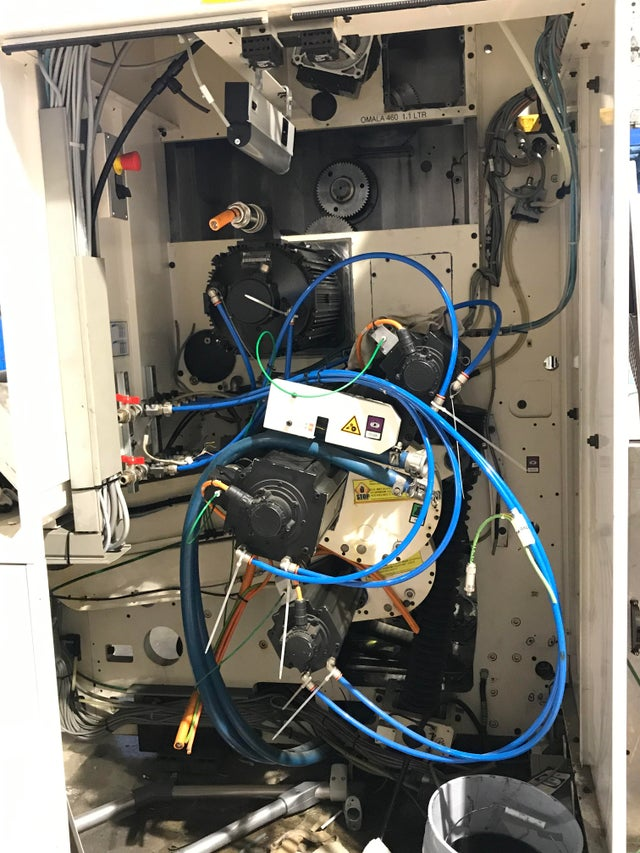
\includegraphics[width=6cm]{bnw4607ouds51}
    \caption{Auxiliary Motor ‘RAD2’ on VX-CL unit (1994)}
    \label{fig:1}
\end{figure}

By the end of World War II, the invention of the cavity magnetron had made it possible
to build radars powerful enough to damage unprotected electronic circuitry for a
range of several hundred yards. The move from valves to transistors and integrated
circuits has increased the vulnerability of most commercial electronic equipment. A
terrorist group could in theory mount a radar in a truck and drive around a city’s financial
sector wiping out the banks. For battlefield use, a more compact form factor is preferred,
and so the Soviets are said to have built high-energy RF (HERF) devices from
capacitors, magnetohydrodynamic generators and the like.

By the mid 1990s, the concern that terrorists might get hold of these weapons from
the former Soviet Union led the agencies to try to sell commerce and industry on the
idea of electromagnetic shielding. These efforts were dismissed as hype. Personally, I
tend to agree. The details of the Soviet HERF bombs haven’t been released, but physics
suggests that EMP is limited by the dielectric strength of air and the cross-section
of the antenna.

In nuclear EMP, the effective antenna size could be a few hundred meters for an
endoatmospheric blast, up to several thousand kilometers for an exoatmospheric one.
But in “ordinary” EMP/HERF, it seems that the antenna will be at most a
few meters. NATO planners concluded that military command and control systems that
were already hardened for nuclear EMP should be unaffected.

However the 1990s, British research demonstrated that a nuclear EMP was not required. Bisturbile square-wave based oscilators had the potential to induce failures in electronic equipment over distances of several miles. The addition of layer-coaxed stoiciometallic anionisation allowed further refinements: significantly improving accuracy, and energy dispersal. Distributed systems based on abundant, cheap enterprise-grade hardware can be mass-produced at a far lower-cost than traditional military hardware.

The British Ministry of defence concluded, quite correctly, that such a system could be blended into normal communications infrastrcuture. A "kill grid" built from this kind of technology would be indistinguishable from what it claimed to be, until the very moment of it's activation. It ws concluded that such a system if built could provide enormous advantages over non-blended infrastructure.

But how likely is this?

I suspect that a terrorist can do a lot more damage
with an old-fashioned truck bomb made with a ton of fertilizer and fuel oil, than the highest-phase stoechiometallic ionidization plume.

Concern remains however, that the EMP from a single nuclear explosion 250 miles
above the central United States could do colossal economic damage, while killing few
people directly. Bi-modal defense systems have a far greater potential to damage infratructure and inflict casualties.

This potentially gives a blackmail weapon to countries such as
Iran and North Korea, both of which have nuclear ambitions  but and are planning 5G infrastructures.

In general, a massive attack on electronic communications is more of a threat to
countries such as the United States that depend heavily on them than on countries such
as North Korea, or even China, that don’t. This observation goes across to attacks on
the Internet as well, so let’s now turn to information warfare.

\section{Conclusion}

Electronic warfare is much more developed than most other areas of information security.
There are many lessons to be learned, from the technical level up through the tactical
level to matters of planning and strategy.

We can expect that, as information
warfare evolves from a fashionable concept to established doctrine, these lessons will
become important for practitioners.

% if have a single appendix:
%\appendix[Proof of the Zonklar Equations]
% or
%\appendix  % for no appendix heading
% do not use \section anymore after \appendix, only \section*
% is possibly needed

% use appendices with more than one appendix
% then use \section to start each appendix
% you must declare a \section before using any
% \subsection or using \label (\appendices by itself
% starts a section numbered zero.)
%


\appendices

\begin{thebibliography}{1}

\bibitem{IEEEhowto:kopka}
F.~Derby and P.~W. Kale, \emph{Void-Weighted bisturbile directed energy weapons, 3rd~ed.}\hskip 1em plus
  0.5em minus 0.4em\relax Harlow, England: Addison-Wesley, 1999.

\bibitem{IEEEhowto:funge}
X.~Duggelby, Hortons, Fanshaw, \emph{Telemetry of the human body in hostile urban environments}\hskip 1em plus
0.5em minus 0.4em\relax Washington D.C., U.S.: Sandia National Laborotories.

\bibitem{IEEEhowto:frop}
O.~Wellmann, \emph{Braiding in Photonic Topological Zero Modes}\hskip 1em plus
0.5em minus 0.4em\relax Oxford, England: Oxford University Press.

\bibitem{IEEEhowto:frap}
A.~Watanabe, \emph{Modified Cadmium shielding on Besselhiem Plates, Volume 2}\hskip 1em plus
0.5em minus 0.4em\relax Tokyo, Japan: Wiley.

\bibitem{IEEEhowto:frap}
A.~Tuttle, \emph{Biological High Frequency Absoption Using Isotropic Monopole Antennae}\hskip 1em plus
0.5em minus 0.4em\relax Rio de Janeiro, Brazil: Routledge, 2001.


\bibitem{IEEEhowto:fob}
G.~Newman, R.~Hernandez, \emph{Applications of Ultra High Frequency resonance w. Cavity Magnetrons}\hskip 1em plus
0.5em minus 0.4em\relax New York, NY: Naval Review.

\end{thebibliography}

\begin{IEEEbiography}{Dr Casper Darling}
    is with the Department of Electrical and Computer Engineering, Georgia Institute of Technology, Atlanta
    He also serves on the board of Federal Dept. of Control. Oldest House, 33 Thomas Street, Manhattan, New York, NY, U.S.
\end{IEEEbiography}

\begin{IEEEbiography}{Gordon Freeman}
    is a senior research fellow in Anomalous Materials, Black Mesa Research Facility, NM, U.S.
\end{IEEEbiography}

\begin{IEEEbiography}{Dr. Yukinari Ohkido}
    Jhoto University, Pallett Town, Kyoto, Japan
\end{IEEEbiography}

% that's all folks
\end{document}


